\begin{figure}[h]
    \begin{subfigure}[b]{0.48\textwidth}
        \centering
	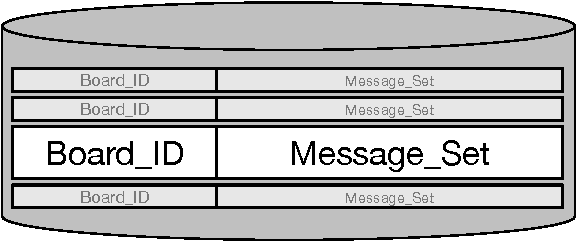
\includegraphics[scale = 0.5]{Figures/SimpleBulletinApp.pdf}
        \caption{Simple Data Model}
    \end{subfigure} 
    \begin{subfigure}[b]{0.48\textwidth}
        \centering
	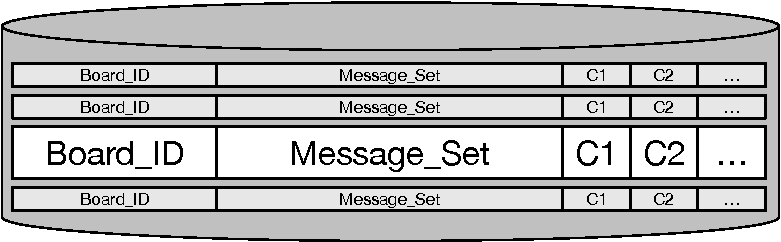
\includegraphics[scale=0.5]{Figures/ModifiedBulletinBoard.pdf}
	\caption{Modified Data Model}
    \end{subfigure}
    \\ \hrulefill \\
\caption{Low-Level Data Model of a Simple Bulletin Board Application
(Left) and the Modified Version Including Session Counters to be Used
for Providing }

\end{figure}
